\documentclass[12pt]{article}

\title{ Introduction to Inflation Theory and its simplest model, Starobinsky Inflation }
\date{Department of Physics, Tokyo Metropolitan University}
\author{Max Miyazaki, 21121003}

\usepackage{amsmath}
\usepackage{amssymb}
\usepackage{ascmac}
\usepackage{amsfonts}
\usepackage{color}
\usepackage[dvipdfmx]{graphicx}
\usepackage{float}
\usepackage{bm}
\usepackage{tcolorbox}
\usepackage{tikz}
\usetikzlibrary{decorations.markings}
\usepackage{indentfirst}
\usepackage[dvipdfmx]{hyperref}
\hypersetup{%
 setpagesize=false,
 bookmarksnumbered=true,
 colorlinks=true,
 linkcolor=blue}



% Define braket-like commands
\newcommand{\bra}[1]{\left\langle #1\right|}
\newcommand{\ket}[1]{\left|#1\right\rangle}
\newcommand{\braket}[2]{\left\langle #1\middle|#2\right\rangle}
\newcommand{\brakets}[3]{\left\langle #1\middle| #2 \middle|#3 \right\rangle}

\newcommand{\tcb}[2]{\begin{tcolorbox}[title={\textcolor{white}{#1}}, opacitybacktitle = 0, colframe=white!40!black]#2
\end{tcolorbox}}

\renewcommand{\arraystretch}{2.1}

\numberwithin{equation}{section}


\begin{document}
\maketitle
\vspace{1cm}
\begin{abstract}
    This paper provides an overview of the standard Big Bang cosmology and its associated problems, followed by an introduction to the concept of inflation. I will show the conditions that must be satisfied for inflation. And since various theoretical models of inflation are considered, I will introduce some representative models and confirm that the models are tightly constrained by cosmological observations. $R^2$ inflation is a good candidate for inflation model that satisfies the restriction. Finally, I briefly discuss how $f(R)$ gravity can avoid instabilities related to ghosts and tachyons.
\end{abstract}

\newpage
\tableofcontents
\newpage
\section{Introduction}
 The Big Bang theory predicts a homogeneous and isotropic universe on large scales, the abundances of light elements, and Cosmic Microwave Background (CMB) radiation. It is an excellent theory, demonstrating high precision and strong agreement between theoretical predictions and observational results \cite{Planck:2018vyg}\cite{BICEP:2021xfz}\cite{Cyburt:2015mya}. However, the theory faces unresolved issues such as the Flatness Problem, Horizon Problem, Monopole Problem, and others. To address these challenges, cosmological inflation was proposed by Linde \cite{Linde:1981mu}, Sato \cite{Sato:1980yn}, Guth \cite{Guth:1980zm}, Kazanas \cite{Kazanas:1980tx}, and others. Inflation assumes that the universe underwent a phase of exponential expansion before the Big Bang. This paradigm is now regarded as a critical component in the early universe's evolution, as it not only resolves the flatness, horizon, and monopole problems, but also addresses domain structure issues \cite{SATO198166}, the gravitino problem \cite{Weinberg:1982zq}, and the origin of the density fluctuations \cite{Hawking:1982cz} observed by the Cosmic Background Explorer (COBE) \cite{COBE:1992syq}. Various inflation models have been proposed, but precise CMB observations have ruled out many of them \cite{Martin:2013tda}. Among the remaining viable models, the Starobinsky inflation model, introduced by A. A. Starobinsky in 1980 \cite{Starobinsky:1980te}, stands out. This model is based on a modified gravity framework, where $f(R) = R + \alpha_{n}R^n$ for $n=2$. Its predictions align with current observations, particularly regarding the power spectrum of primordial curvature perturbations and the spectrum of primordial gravitational waves \cite{Alam:2024kgk}\cite{German:2023euc}. Moreover, the Starobinsky inflation model is closely tied to supergravity theory, a low-energy effective field theory emerging from superstring theory \cite{Ketov2024}. While supergravity can naturally generate inflation \cite{Kallosh:2010ug}, incorporating the Starobinsky model and its extensions allows for consistency with observations and facilitates the exploration of a deeper, more fundamental theory of inflation. Thus, the Starobinsky model serves as an essential tool for advancing our understanding of high-energy physics and quantum gravity.\par
 Finally, I would like to list some of the books that I consulted in writing this paper \cite{matsubara_cos1}\cite{matsubara_cos2}\cite{matsubara_base}\cite{tsujikawa_cos}\cite{Weinberg_cos}.

\section{Standard Big Bang Theory}
\subsection{Cosmological principle}
The standard model of modern cosmology is built upon the assumption of the cosmological principle, which is stated as follows:
\tcb{Cosmological principle}{\textbf{The universe is homogeneous and isotropic on large-scale.}\par
Homogeneous: the universe looks the same from all points in space.\par
Isotropic: the universe looks the same in all directions.}
\noindent Of course, the universe exhibits hierarchical structures on both small and large scales, so the assumptions of homogeneity and isotropy do not apply at scales where these structures are visible. However, when averaged over sufficiently large scales, we accept as a principle that the universe has no special location or direction.

\subsection{FLRW metric}
Assuming the cosmological principle leads to the FLRW metric $g_{\mu\nu}$  which describes the space-time structure of the universe
\begin{equation}\label{flrw m}
    g_{\mu\nu} = \begin{pmatrix}
        -1 & 0 & 0 & 0\\
        0 & \dfrac{a^2(t)}{1 - kr^2} & 0 & 0\\
        0 & 0 & a^2(t)r^2 & 0\\
        0 & 0 & 0 & a^2(t)r^2\sin^2\theta
    \end{pmatrix},
\end{equation}
the inverse metric $g^{\mu\nu}$ is
\begin{equation}\label{flrw im}
    g^{\mu\nu} = \begin{pmatrix}
        -1 & 0 & 0 & 0\\
        0 & \dfrac{1 - kr^2}{a^2(t)} & 0 & 0\\
        0 & 0 & \dfrac{1}{a^2(t)r^2} & 0\\
        0 & 0 & 0 & \dfrac{1}{a^2(t)r^2\sin^2\theta}
    \end{pmatrix}.
\end{equation}
Therefore, the square of the spacetime interval $ds^2$ is,
\begin{align}
    ds^2 &= -dt^2 + a^2(t)\left( \frac{dr^2}{1 - kr^2} + r^2(d\theta^2 + \sin^2\theta d\phi^2) \right)\\
    &= -dt^2 + a^2(t)\gamma_{ij}dx^{i}dx^{j}.
\end{align}
Where $\gamma_{ij}$ is a time-independent 3-dimensional homogeneous and isotropic metric, $\gamma_{11} = \displaystyle \frac{1}{1 -kr^2}$, $\gamma_{22} = r^2$, $\gamma_{33} = r^2\sin^2\theta$, $\gamma_{ij} = 0 \hspace{0.3cm} (i \neq j)$. Here, $a(t)$ is the scale factor,  which depends only on time, and $k$ is the curvature parameter, defined as follows:
\begin{equation}\label{curvature parameter}
k = \begin{cases} 
-1, & \textrm{Closed space.} \\ 
0, & \textrm{Flat space.} \\ 
+1, & \textrm{Open space.} 
\end{cases}
\end{equation}
And an important quantity characterizing the FLRW spacetime is the \textit{Hubble constant} $H$, which represents the expansion rate of spacetime. It is defined as
\begin{equation}\label{Hubble const def}
    H \equiv \frac{\dot{a}}{a} \hspace{0.5cm} \left(\dot{a} \equiv \frac{da}{dt}\right).
\end{equation}


\subsection{Einstein field equations}
The action $S$ that yields the Einstein field equations is given by
\begin{equation}\label{EFTA}
    S = \int \left[ \frac{1}{2\kappa^2}\left( R - 2\Lambda \right) + \mathcal{L}_{\textrm{matter}} \right]\sqrt{-g}\, d^4x.
\end{equation}
Here, $\kappa^2$ is a constant given by $\kappa^2 = \displaystyle \frac{8\pi G}{c^4} = \frac{1}{M_{\textrm{Pl}}^2}$. (See \eqref{S Planck mass} for $M_{\textrm{Pl}}$).\\
$\Lambda$ is the cosmological constant.\\
$g$ denotes the determinant of the metric tensor matrix, $g = \det(g_{\mu\nu})$.\\
$R$ is Ricci scalar, defined as
\begin{equation}\label{Ricci scalar def}
    R = g^{\mu\nu}R_{\mu\nu},
\end{equation}
where $R_{\mu\nu}$ is Ricci curvature tensor,  expressed as
\begin{equation}\label{Ricci tensor def}
    R_{\mu\nu} = \frac{\partial{\Gamma^{\alpha}}_{\mu\nu}}{\partial x^\alpha} - \frac{\partial{\Gamma^{\alpha}}_{\mu\alpha}}{\partial x^\nu} + {\Gamma^{\alpha}}_{\beta\alpha}{\Gamma^{\beta}}_{\mu\nu} - {\Gamma^{\alpha}}_{\beta\nu}{\Gamma^{\beta}}_{\mu\alpha},
\end{equation}
and ${\Gamma^{\alpha}}_{\mu\nu}$ are the Christoffel symbols, defined as
\begin{equation}\label{Christoffel def}
    {\Gamma^{\alpha}}_{\mu\nu} \equiv \frac{1}{2}g^{\alpha\beta}\left( \frac{\partial g_{\beta\mu}}{\partial x^\nu} + \frac{\partial g_{\beta\nu}}{\partial x^\mu} - \frac{\partial g_{\mu\nu}}{\partial x^\beta} \right).
\end{equation}
Using the principle of stationary action $\delta S = 0$, Einstein field equations are derived as
\begin{equation}\label{EFE}
    R_{\mu\nu} -\frac{1}{2}g_{\mu\nu}R + \Lambda g_{\mu\nu}= \frac{8\pi G}{c^4}T_{\mu\nu}.
\end{equation}
The energy-momentum tensor $T_{\mu\nu}$ for a perfect fluid is used, as the universe is assumed to be homogeneous and isotropic:
\begin{equation}\label{EMT of pfluid}
    T_{\mu\nu} = \begin{pmatrix}
        \rho c^2 & 0 & 0 & 0\\
        0 & p & 0 & 0\\
        0 & 0 & p & 0\\
        0 & 0 & 0 & p\\
    \end{pmatrix},
\end{equation}
where $\rho$ is the mass density, $\rho c^2$ is the energy density, and $p$ is the pressure.

\subsection{Geometric quantities}
From \eqref{flrw m} and \eqref{flrw im}, the components of the FLRW metric are given by
\begin{align}\label{flrw component}
    g_{00} &= -1,\hspace{0.3cm} g_{11} = \frac{a^2}{1 - kr^2},\hspace{0.3cm} g_{22} = a^2 r^2,\hspace{0.3cm} g_{33} = a^2 r^2 \sin^2\theta, \notag\\
    g^{00} &= -1,\hspace{0.3cm} g^{11} = \frac{1 - kr^2}{a^2},\hspace{0.3cm} g^{22} = \frac{1}{a^2 r^2},\hspace{0.3cm} g^{33} = \frac{1}{a^2 r^2 \sin^2\theta}.
\end{align}
Substituting \eqref{flrw component} into \eqref{Christoffel def}, we obtain the non-zero components of the Christoffel symbols as follows:
\begin{align}\label{Christoffel component}
   {\Gamma^{0}}_{11} &= \frac{a\dot{a}}{c}\frac{1}{1 - kr^2},\hspace{0.3cm} {\Gamma^{0}}_{22} = \frac{a\dot{a}}{c}r^2,\hspace{0.3cm} {\Gamma^{0}}_{33} = \frac{a\dot{a}}{c}r^2\sin^2\theta, \notag\\
   {\Gamma^{1}}_{11} &= \frac{kr}{a - kr^2},\hspace{0.3cm} {\Gamma^{1}}_{22} = -(1 - kr^2)r,\hspace{0.3cm} {\Gamma^{1}}_{33} = -(1 - kr^2)r\sin^2\theta, \notag\\
   {\Gamma^{1}}_{01} &= {\Gamma^{1}}_{10} = {\Gamma^{2}}_{02} = {\Gamma^{2}}_{20} = {\Gamma^{3}}_{02} = {\Gamma^{3}}_{30} = \frac{1}{c}\frac{\dot{a}}{a}, \notag\\
   {\Gamma^{2}}_{12} &= {\Gamma^{2}}_{21} = {\Gamma^{3}}_{31} = {\Gamma^{3}}_{13} = \frac{1}{r}, \notag\\
   {\Gamma^{2}}_{33} &= -\sin\theta\cos\theta,\hspace{0.3cm} {\Gamma^{3}}_{32} = {\Gamma^{3}}_{23} = \frac{\cos\theta}{\sin\theta}.
\end{align}
In the same way, substituting \eqref{Christoffel component} into \eqref{Ricci tensor def}, we obtain the non-zero components of the Ricci curvature tensor. Using these, the Ricci scalar, as defined in \eqref{Ricci scalar def}, can also be determined.
\begin{align}\label{Ricci tensor component}
    R_{00} &= -\frac{3}{c^2}\frac{\ddot{a}}{a} \notag\\
    R_{11} &= \frac{1}{c^2}\frac{a\ddot{a} + 2\dot{a}^2 + 2kc^2}{1 - kr^2} \notag\\
    R_{22} &= \frac{1}{c^2}(a\ddot{a} + 2\dot{a}^2 + 2kc^2)r^2 \notag\\
    R_{33} &= \frac{1}{c^2}(a\ddot{a} + 2\dot{a}^2 + 2kc^2)r^2\sin^2\theta \notag\\
    R &= \frac{6}{c^2}\frac{a\ddot{a} + \dot{a}^2 + kc^2}{a^2}.
\end{align}

\subsection{Friedmann equation}
Assume that space-time is homogeneous and isotropic (FLRW metric \eqref{flrw m}) and that the matter distribution is like a perfect fluid \eqref{EMT of pfluid}. Let's solve the Einstein field equations under these conditions.\par
First, let's examine the $00$ component of \eqref{EFE},
\begin{align*}
    R_{00} -&\frac{1}{2}Rg_{00} -\Lambda g_{00} = \frac{8\pi G}{c^4}T_{00} \notag\\
    -\frac{3}{c^2}\frac{\ddot{a}}{a} -\frac{1}{2}&\left( \frac{6}{c^2}\frac{a\ddot{a} + \dot{a}^2 + kc^2}{a^2} \right)(-1)+\Lambda (-1) = \frac{8\pi G}{c^4}(\rho c^2) \notag\\
    &\frac{\dot{a}^2 + kc^2}{a^2} = \frac{8\pi G\rho + \Lambda c^2}{3}.
\end{align*}
This is called the first Friedmann equation and represents the rate of expansion of the universe.
\tcb{First Friedmann equation (universe expansion rate)}{
    \begin{equation}\label{Friedmann eq1}
        \frac{\dot{a}^2 + kc^2}{a^2} = \frac{8\pi G\rho + \Lambda c^2}{3}
    \end{equation}
    \hspace{2cm}or using \eqref{Hubble const def},
    \begin{equation}\label{Friedmann eq1_H}
        H^2 = \frac{8\pi G\rho + \Lambda c^2}{3} -\frac{kc^2}{a^2}.
    \end{equation}
}
\noindent Next, take the trace of \eqref{EFE},
\begin{align*}
    R_{\mu\nu}g^{\mu\nu} -\frac{1}{2}Rg_{\mu\nu}g^{\mu\nu} &+ \Lambda g_{\mu\nu}g^{\mu\nu} = \frac{8\pi G}{c^4}T_{\mu\nu}g^{\mu\nu}\\
    &-R + 4\Lambda = \frac{8\pi G}{c^4}T\\
    -\frac{6}{c^2}\frac{a\ddot{a} + \dot{a}^2 + kc^2}{a^2} &+ 4\Lambda = \frac{8\pi G}{c^4}(-\rho c^2 + 3p)\\
    \frac{\ddot{a}}{a} + \frac{\dot{a}^2 + kc^2}{a^2} &-\frac{2}{3}\Lambda c^2 = \frac{4\pi G}{3c^2}(\rho c^2 -3p)\\
    \frac{\ddot{a}}{a} + \frac{8\pi G\rho + \Lambda c^2}{3} &-\frac{2}{3}\Lambda c^2 = \frac{4\pi G}{3c^2}(\rho c^2 -3p)\\
    \frac{\ddot{a}}{a} = -&\frac{4\pi G}{3}\left( \rho + \frac{3p}{c^2} \right) + \frac{\Lambda c^2}{3}.
\end{align*}
This is called the Raychaudhuri equation and represents the acceleration of the universe.
\tcb{Raychaudhuri equation (universe acceleration rate)}{
    \begin{equation}\label{Friedmann eq2}
        \frac{\ddot{a}}{a} = -\frac{4\pi G}{3}\left( \rho + \frac{3p}{c^2} \right) + \frac{\Lambda c^2}{3}
    \end{equation}
}
\eqref{Friedmann eq1} (or \eqref{Friedmann eq1_H}), \eqref{Friedmann eq2} are the equations for the expansion of the universe in the standard Big Bang theory. Differentiating \eqref{Friedmann eq1} with respect to time and substituting \eqref{Friedmann eq2}, we obtain the conservation law
\begin{equation}\label{Friedmann eq3}
    \dot{\rho} = -3\frac{\dot{a}}{a}\left( \rho + \frac{p}{c^2} \right).
\end{equation}
This is also confirmed by the fact that it is derived from the local conservation of the energy-momentum tensor:
\begin{equation}
    \nabla_\mu T^{\mu\nu} = 0.
\end{equation}
The Friedmann equations cannot be solved as they are because there are three unknown variables: $a(t)$, $\rho(t)$, and $p(t)$. Therefore, the matter or energy component in the universe is determined by the equation of state. 
\tcb{Equation of state}{
    \begin{equation}\label{EoS}
        p = w\rho c^2, \hspace{0.3cm} \textrm{$w$ : parameter}.
    \end{equation}
    \hspace{0.3cm} Dust-like matter : $w = 0 \to p=0$.\\
    \hspace{0.3cm} Radiation : $w = \displaystyle \frac{1}{3} \to p = \frac{1}{3}\rho c^2$.\\
    \hspace{0.3cm} Dark energy : $w = -1 \to p = -\rho c^2$.
}
Substituting \eqref{EoS} into \eqref{Friedmann eq3} and solving, we obtain the following relation:
\begin{equation}
    \rho \propto a^{-3(1 + w)}.
\end{equation}
Using this result in \eqref{Friedmann eq1}, we obtain the time dependence of $a(t)$ for each state of the universe. To summarize these results,
\begin{table}[H]
    \centering
    \begin{tabular}{|c|c|c|c|}\hline
        Type of universe & $w$-parameter & $\rho$ - $a$ relation & $a$ - $t$ relation \\ \hline
        Matter & $w = 0$ & $\rho \propto a^{-3}$ & $a(t) \propto \displaystyle t^{-\frac{2}{3}}$\\ \hline
        Radiation & $w = \displaystyle \frac{1}{3}$ & $\rho \propto a^{-4}$ & $a(t) \propto \displaystyle t^{-\frac{1}{2}}$\\ \hline
        Dark energy ($\Lambda$) & $w = -1$ & $\rho \propto 1 $ & $a(t) \propto \displaystyle \exp {\sqrt{\frac{\Lambda}{3}}ct}$\\ \hline
    \end{tabular}
    \caption{Each universe type}\label{table of universe type}
\end{table}

\subsection{Cosmological observations}
Cosmological parameters in observational cosmology are derived from the Friedmann equation. The mass density when there is no cosmological constant ($\Lambda = 0$) and the curvature of the universe is zero ($k = 0$) is called the \textit{critical density} $\rho_c$. We can define a density parameter $\Omega_{\textrm{M/R}}$
\begin{equation}
    \Omega_{\textrm{M/R}} \equiv \frac{\rho}{\rho_c}.
\end{equation}
Substituting in \eqref{Friedmann eq1} with $\rho \to \rho_c$ ($\Lambda = 0, k = 0$), we get:
\begin{align}
    \frac{\dot{a}^2}{a^2} &= \frac{8\pi G \rho_c}{3} \notag\\
    H^2 &= \frac{8\pi G \rho_c}{3} \notag\\
    \rho_c &= \frac{3H^2}{8\pi G}.
\end{align}
Therefore, the density parameter is obtained as
\begin{equation}
    \Omega_{\textrm{M/R}} \equiv \frac{\rho}{\rho_c} = \frac{8\pi G}{3H^2}\rho.
\end{equation}
Now rewrite Friedmann equation \eqref{Friedmann eq1_H} as follows:
\begin{align}
    H^2 &= \frac{8\pi G\rho + \Lambda c^2}{3} -\frac{kc^2}{a^2} \notag\\
    1 &= \frac{8\pi G}{3H^2}\rho -\frac{kc^2}{a^2 H^2} + \frac{\Lambda c^2}{3H^2}.
\end{align}
Here, the following two parameters are defined:
\vskip\baselineskip
\noindent Curvature parameter
\begin{equation}
    \Omega_{k} \equiv -\frac{kc^2}{a^2 H^2}
\end{equation}
Dark energy parameter
\begin{equation}
    \Omega_{\Lambda} \equiv \frac{\Lambda c^2}{3H^2}.
\end{equation}
Using these parameters, the Friedmann equation is rewritten as
\tcb{Friedmann equation (Parameter representation)}{
    \begin{equation}\label{Friedmann eq rewrite}
        1 = \Omega_{\textrm{M/R}} + \Omega_{k} + \Omega_{\Lambda}.
    \end{equation}
}
In 1998, observations confirmed that the universe is accelerating and expanding ($\Lambda > 0$) \cite{Peebles:2002gy}. These parameters were confirmed to agree with theoretical values with high precision through observations by WMAP \cite{BICEP:2021xfz}, BOOMERanG \cite{Masi:2002hp}, Planck \cite{Planck:2018vyg}, and others. Other observations of the formation of cosmic structure and the abundance of light elements are also consistent with the predictions of the Big Bang theory \cite{Lyth:2009zz}. With such observational support, the Big Bang theory was established as the standard model of modern cosmology.

\section{Inflation}
\subsection{Big Bang's problem}
In the previous section, I introduced the Standard Big Bang theory as a successful framework of modern cosmology. However, some aspects cannot be explained by the Big Bang theory.
\tcb{Problems of the Big Bang Model}{
    \begin{itemize}
        \item Flatness Problem
        \item Horizon Problem
        \item Monopole Problem
    \end{itemize}
}

\subsection*{Flatness Problem}
From \eqref{Friedmann eq rewrite},
\begin{equation}
    \Omega_k = 1 - (\Omega_{\textrm{M/R}} + \Omega_{\Lambda}) = -\frac{kc^2}{a^2 H^2}.
\end{equation}
If $k \neq 0$, $\Omega_k$ affects the change in the scale factor and significantly alters the flatness of the universe. In order to maintain the current flatness value $\Omega_k = 0.0007 \pm 0.0019\hspace{0.2cm}(68\%\,\textrm{CL,\, TT,TE,EE+lowE+lensing+BAO})$ \cite{Planck:2018vyg}, the initial conditions must be very precisely controlled in the early universe, and the Big Bang theory can only explain this as a coincidence.

\subsection*{Horizon Problem}
The currently observed CMB is very homogeneously distributed, and its temperature is nearly constant ($T \approx 2.7 \textrm{K}$) \cite{Planck:2018vyg}\cite{BICEP:2021xfz}. It is unnatural for the temperature to be homogeneous in two distant and separate regions because they cannot causally interact with each other at the normal rate of cosmic expansion.

\subsection*{Monopole Problem}
A particle with a single magnetic charge is called a magnetic monopole. Although monopoles are predicted to be produced in large numbers at the energy scale of Grand Unified Theories (GUTs) \cite{tHooft:1974kcl}, such as in the early universe, current observations indicate that no monopoles have been observed in the universe.

\subsection*{Other Problems}
There are other problems, such as the Primordial Lithium Problem and the Baryon Asymmetry Problem, but these are still unsolved issues that are the subject of various studies. See \cite{Fields:2011zzb}\cite{Bernreuther:2002uj} for more information.

\subsection{Problem solving by introducing Inflation}
The Flatness and Horizon problems can be solved by considering Inflation, in which the early universe expanded exponentially in a very short period of time \cite{Guth:1980zm}. In fact, in the case of the Flatness Problem, the exponential expansion of the universe causes the curvature term $\Omega_k$ to rapidly approach zero, so that whatever curvature the universe has under initial conditions will result in a flat universe at the current time. In the case of the Horizon Problem, the exponential expansion of the early universe allows regions that would not normally be able to causally interact with each other to do so before the expansion. In the case of the Monopole Problem, monopoles that existed in large numbers in the early universe become extremely sparse due to exponential expansion and result in densities that are undetectable in the currently observable universe. Here, we evaluate quantitatively how long inflation should last. Let $a(t_i) = a_i$ be the scale factor at time $t_i$ when inflation starts, and $a(t_f) = a_f$ at the end time $t_f$. The expansion index at any time $t$ during inflation is defined as follows and is called the \textit{e-folding number} $N$,
\tcb{e-folding number}{
    \begin{equation}\label{e-folding_def}
        N(t) \equiv \log\left( \frac{a_f}{a(t)} \right) = \int_{t}^{t_f} H dt.
    \end{equation}
}
\noindent This $N(t)$ is often used as a quantity to characterize how long the inflationary period lasted after a certain time $t$. It is known that the flatness and horizon problems can be solved with $N \geq 50$ \cite{Riotto:2002yw}. The total expansion index throughout the entire inflationary period is defined as 
\begin{equation}
    \mathcal{N} \equiv N(t_i)
\end{equation}
In other words, 
\begin{equation}
    \frac{a_f}{a_i} = e^{\mathcal{N}}.
\end{equation}
There is no significant change in the total amount of e-folds, the value of total e-foldings is ranged from $50-70$ \cite{Lyth:1998xn}.

\subsection{Scalar Field Dynamics}
Consider constructing an inflation model from a field theory perspective. Without specifying the physical properties, we use a scalar field $\phi$, called the \textit{inflaton}, as the order parameter to parameterize the time evolution of the energy density during inflation. Considering a simple model with a scalar potential of $V(\phi)$ and a single scalar field, the Lagrangian $\mathcal{L}_{\textrm{matter}}$ is 
\begin{equation}
    \frac{1}{\sqrt{-g}}\mathcal{L}_{\textrm{matter}} = \frac{1}{2}g^{\mu\nu}\partial_{\mu}\phi \partial_{\nu}\phi - V(\phi).
\end{equation}
From \eqref{EFTA},
\begin{align}
    S &= \int \left[ \frac{1}{2\kappa}\left( R - 2\Lambda \right)\sqrt{-g} + \mathcal{L}_{\textrm{matter}} \right]\, d^4x \notag\\
    &= \int \left[ \frac{1}{2\kappa}\left( R - 2\Lambda \right) + \frac{1}{2}g^{\mu\nu}\partial_{\mu}\phi \partial_{\nu}\phi - V(\phi) \right]\sqrt{-g}\, d^4x\notag\\
    &= S_{\textrm{EH}} + S_{\phi}
\end{align}
The action $S$ is the sum of the Einstein-Hilbert action $S_{\textrm{EH}}$, and the action of a scalar field with a canonical kinetic term,
\begin{equation}
    S_{\phi} \equiv \int \mathcal{L}_{\textrm{matter}}\,d^4 x.
\end{equation}
The potential $V(\phi)$ describes the self-interactions of the scalar field. Since the energy-momentum tensor is defined by
\begin{equation}
    T_{\mu\nu} \equiv -\frac{2}{\sqrt{-g}}\frac{\delta (\sqrt{-g}S_\phi)}{\delta g^{\mu\nu}},
\end{equation}
the energy-momentum tensor for the scalar field is
\begin{equation}
    T_{\mu\nu}^{(\phi)} = \partial_\mu \phi \partial_\nu \phi - g_{\mu\nu}\left(  \frac{1}{2}\partial^\sigma \phi \partial_\sigma \phi + V(\phi) \right).
\end{equation}
Suppose the FLRW metric \eqref{flrw m}, where $T_{\mu\nu}$ is the energy-momentum tensor of the perfect fluid \eqref{EMT of pfluid}, and $\phi$ depends only on time $\phi(t, \bm{x}) \equiv \phi(t)$. Then, we have 
\begin{align}
    \rho c^2 &= \frac{1}{2}\dot{\phi}^2 + V(\phi),\\
    p &= \frac{1}{2}\dot{\phi}^2 - V(\phi).
\end{align}
Substituting these results into the energy conservation law \eqref{Friedmann eq3} and the Friedmann equations \eqref{Friedmann eq1_H} and \eqref{Friedmann eq2}, we get
\begin{equation}\label{ECL_phi}
    \ddot{\phi} + 3H\dot{\phi} + \frac{dV}{d\phi} = 0,
\end{equation}
\begin{equation}\label{Friedmann1_phi}
    H^2 = \frac{8\pi G}{3c^2}\left( \frac{1}{2}\dot{\phi}^2 + V(\phi) \right),
\end{equation}
\begin{equation}\label{Friedmann2_phi}
    \dot{H} = -\frac{4\pi G\dot{\phi}}{c^2}.
\end{equation}
Here, the role of the cosmological constant $\Lambda$ is substituted by the potential $V(\phi)$ of the inflaton field during the inflationary period. Also, during the inflationary period, the contribution of the curvature term $\Omega_k$ becomes very small $(\Omega_k \to 0)$ because the scale factor increases exponentially.

\subsection{Slow-Roll conditions}
The term $3H\dot{\phi}$ in \eqref{ECL_phi} can be viewed as a friction term. If the value of $V(\phi)$ is large, then H is also large from \eqref{Friedmann1_phi}. This also makes the friction term larger, and the scalar field can be seen as slowly rolling through the potential. In other words, the expansion of the universe acts to prevent changes in the scalar field. This allows the scalar field values to change slowly enough while the universe continues to expand rapidly, provided that the slope $\frac{dV}{d\phi}$ of the potential is small enough. In this case, the acceleration term $\ddot{\phi}$ in \eqref{ECL_phi} is sufficiently small compared to the friction term that, to a good approximation, we have
\begin{equation}\label{ECL_phi_approx}
    \dot{\phi} \simeq -\frac{1}{3H}\frac{dV}{d\phi}.
\end{equation}
In order for inflation to occur such that this approximation holds, the following two conditions need to be satisfied:
\begin{equation}\label{SR_condition}
    |\dot{\phi}| \ll 2V(\phi),\hspace{0.3cm} |\ddot{\phi}| \ll 3H|\dot{\phi}|.
\end{equation}
A slow change in the value of the scalar field is called \textit{slow-roll}, and this conditional equation is referred to as the \textit{slow-roll condition}. If this condition holds, then \eqref{Friedmann1_phi} is approximately
\begin{equation}\label{Friedmann1_phi_approx}
    H^2 \simeq \frac{8\pi G}{3c^2}V.
\end{equation}
From \eqref{Friedmann2_phi} and \eqref{Friedmann1_phi_approx},
\begin{equation}\label{H_SR}
    \frac{\dot{H}}{H^2} \simeq -\frac{3\dot{\phi}^2}{2V} \ll 1.
\end{equation}
This equation shows that the time variation of $H$ is sufficiently small when the slow-roll condition holds. Rewriting e-folding number \eqref{e-folding_def} using \eqref{ECL_phi_approx} and \eqref{H_SR} yields
\begin{align}\label{e-folding_phi}
    N &= \int_{t}^{t_f} H \,dt \notag\\
    &= \int_{\phi(t)}^{\phi_f} \frac{H}{\dot{\phi}} \,d\phi \notag\\
    &= \int_{\phi(t)}^{\phi_f} H \,\frac{1}{-\frac{1}{3H}\frac{dV}{d\phi}} d\phi \notag\\
    &= \int_{\phi(t)}^{\phi_f} -\frac{3H^2}{\frac{dV}{d\phi}} \notag\\
    &= \int_{\phi(t)}^{\phi_f} -\frac{3}{\frac{dV}{d\phi}}\frac{8\pi G}{3c^2}\, d\phi \notag\\
    &= \frac{8\pi G}{c^2} \int_{\phi_f}^{\phi(t)} \frac{V(\phi)}{\frac{dV}{d\phi}}\, d\phi,
\end{align}
where $\phi_f \equiv \phi(t_f)$ is the value of the scalar field at the end of inflation. About 50-70 e-folds are mentioned as the number of e-folds needed to explain the uniformity of the CMB, but it is generally considered better to have about 55 e-folds to experience enough inflation to explain the observed universe \cite{Remmen:2014mia}. Differentiating \eqref{ECL_phi_approx} with respect to time and using \eqref{H_SR} under the slow-roll conditions \eqref{SR_condition} yields 
\begin{equation}\label{D_ECL_phi_approx}
    \ddot{\phi} \simeq -\frac{\dot{\phi}^2}{2V}\frac{dV}{d\phi} -\frac{\dot{\phi}}{3H}\frac{d^2 V}{d\phi^2}.
\end{equation}
Substituting \eqref{ECL_phi_approx} and \eqref{D_ECL_phi_approx} into \eqref{SR_condition} yields the condition on the potential:
\begin{equation}
    \left( \frac{1}{V}\frac{dV}{d\phi} \right)^2 \ll \frac{48\pi G}{c^2},\hspace{0.3cm} \left| \frac{1}{V}\frac{d^2 V}{d\phi^2} \right| \ll \frac{24\pi G}{c^2}.
\end{equation}
This indicates that the shape of the potential $V(\phi)$ must be very flat. Introduce the following parameters to quantify slow-roll conditions,
\begin{equation}\label{SR_parameter}
    \epsilon_{V} \equiv \frac{M_{\textrm{Pl}}^2}{2}\left( \frac{1}{V}\frac{dV}{d\phi} \right)^2, \hspace{0.3cm} \eta_{V} \equiv M_{\textrm{Pl}}^2\frac{1}{V}\frac{d^2V}{d\phi^2},
\end{equation}
where $M_{\textrm{Pl}}$ is the reduced Planck mass defined as
\begin{equation}\label{S Planck mass}
    M_{\textrm{Pl}} = \frac{1}{\sqrt{8\pi G / \hbar c}} = 2.4 \times 10^{18}\,\textrm{GeV},
\end{equation}
the Planck mass is $M_{\textrm{P}} \equiv \sqrt{c\hbar / G}$. Parameters such as \eqref{SR_parameter} are called the \textit{slow-roll parameters}. Both $\epsilon_{V}$ and $\eta_{V}$ are small numbers under slow-roll conditions $(\epsilon_{V}, \eta_{V} \ll 1)$, and inflation ends at about $\epsilon_{V}, \eta_{V} \simeq 1$. Thereafter, Planck unit system is adopted   $(c = \hbar = k_{\textrm{B}} = 1)$.

\subsection{Typical Inflation Models}
Inflation can be described by various models that share the common feature of causing accelerated expansion in the early universe. Many models have been proposed: \textit{old, new, pre-owned, chaotic, quixotic, ergodic, exotic, heterotic, autoerotic, natural, supernatural, au natural, power-law, powerless, power-mad, one-field, two-field, home-field, modulus, modulo, moduli, self-reproducing, self-promoting, hybrid, low-bred, white-bread, first-order, second-order, new-world order, pre-big-bang, no-big-bang, post-big-bang, D-term, F-term, winter-term, supersymmetric, superstring, superstitious, extended, hyperextended, overextended, D-brane, p-brane, No-brain, dilaton, dilettante}, ect. These different types of models can be broadly categorized \cite{Kolb:1999ar}. Here, some typical models are presented and showing the form of the potential $V(\phi)$.
\subsection*{Large field models}
In this models, the initial value of the inflaton is large and the potential decreases as $\phi$ decreases. Chaotic inflation is one of the representative of large-field models \cite{Linde:1983gd}.
\subsubsection*{Chaotic Inflation}
The Chaotic Inflation model is described by quadratic or quartic inflaton potential:
\begin{equation}
    V(\phi) = \frac{1}{2}m^2 \phi^2,\hspace{0.3cm}\textrm{or}\hspace{0.3cm} V(\phi) = \frac{1}{4}\lambda\phi^4.
\end{equation}
\begin{figure}[H]
    \centering
    \begin{tikzpicture}[scale=1.2]
        % 軸
        \draw[->] (-4,0) -- (4,0) node[below] {$\phi$};
        \draw[->] (0,0) -- (0,4) node[left] {$V(\phi)$};
    
        % カオティックインフレーションのポテンシャル V(phi) = (1/2)m^2 * phi^2
        \draw[thick, blue, samples=100, domain=-3.5:3.5, smooth, variable=\x] 
            plot (\x, {0.2 * \x * \x});
    
        % ポテンシャルを下る様子の矢印
        \draw[->, thick, red] (-2.6,1.4) -- (-2,0.9) node[midway, below left] {\small \textit{Inflation}};
    
        % 最小点付近での単振動を示す矢印
        \draw[<->, thick, orange] (-0.3,0.3) -- (0.3,0.3) node[midway, above] {\small \textit{Oscillations}};
        \fill[red] (0,0.1) circle(3pt);
        \node[below left] at (0.5,0) {\small $\phi=0$};
    
        % ポイントラベル(頂点や曲線上)
        \fill[red] (-2.6,1.5) circle(3pt);
    
        \node[below right] at (3.5,2.45) {\small $V(\phi) = \frac{1}{2}m^2\phi^2$};
    \end{tikzpicture}
    \caption{Chaotic Inflation Potential Diagram for $\displaystyle V(\phi) = \frac{1}{2}m^2 \phi^2$}
\end{figure}
\noindent The term "Chaotic" refers to the idea that the initial conditions of the inflaton are distributed chaotically.
This model is advantageous because the form of the potential is simple. However, most recent CMB measurements ruled out all power-law chaotic models including those in (3.24), see \hyperref[fig:Planck]{Fig.3}.

\subsection*{Small field model}
In this model, the inflaton field is initially small and slowly evolves toward the potential minimum as $\phi$ increases. Natural Inflation and New Inflation \cite{Albrecht:1982wi} are examples of this model.

\subsubsection*{Natural Inflation}
The Natural Inflation model features the pseudo Nambu-Goldstone boson (PNGB) that emerges when an approximate global symmetry is spontaneously broken \cite{Adams:1992bn}.
\tcb{pseudo-Nambu-Goldston boson (pNGB)}{
    Consider a theory where the Lagrangian can be divided into a part invariant under a group $G$ and a small perturbation invariant only under a subgroup of $G$, which introduces explicit symmetry breaking. By setting the perturbation parameter $\epsilon$ to a small but nonzero value, the symmetry of $G$ is spontaneously broken in the limit $\epsilon \to 0$.\\
    In this scenario, the Nambu-Goldstone (NG) modes predicted by Goldstone's theorem acquire a small mass (a nonzero gap) due to the perturbation. Such approximate NG bosons are referred to as pseudo-Nambu-Goldstone Bosons (pNGBs) \cite{Brauner:2024juy}.
}
\noindent This model considers the pNGB that emerges by adding symmetry breaking as an inflaton, with its potential given by
\begin{equation}
    V(\phi) = V_0 \left( 1 + \cos\left( \frac{\phi}{f} \right) \right),
\end{equation}
where $f$ denotes the scale for symmetry breaking.
\begin{figure}[H]
    \centering
    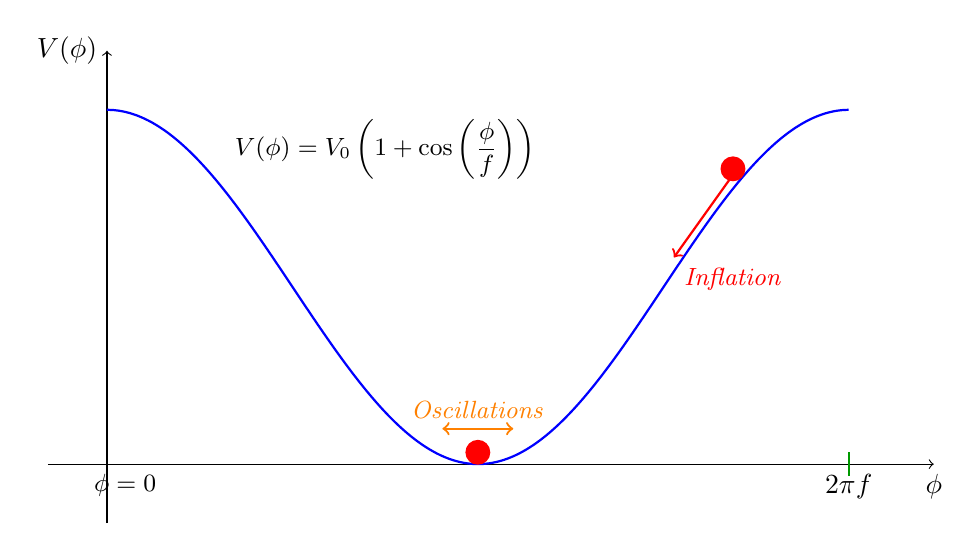
\begin{tikzpicture}[scale=1.5]

        % 軸
        \draw[->] (-0.5,0) -- (7,0) node[below] {$\phi$};
        \draw[->] (0,-0.5) -- (0,3.5) node[left] {$V(\phi)$};
        
        % ポテンシャル V(φ) = 1 + cos(φ/f)
        \draw[thick, blue, domain=0:6.28, samples=100, smooth] 
            plot (\x,{1.5*(1 + cos(deg(\x)))});
        
        % 軸の目盛り
        \node[below] at (6.28,0) {$2\pi f$};
        \draw[thick, green!60!black] (6.28,-0.1) -- (6.28,0.1); % 緑色の目盛り

        % 最小点付近での単振動を示す矢印
        \draw[<->, thick, orange] (2.84,0.3) -- (3.44,0.3) node[midway, above] {\small \textit{Oscillations}};
        \fill[red] (3.14,0.1) circle(3pt);
        \node[below left] at (0.5,0) {\small $\phi=0$};
    
        % ポテンシャル上の赤い点
        \fill[red] (5.3,2.5) circle (3pt);
        \draw[->, thick, red] (5.3,2.45) -- (4.8,1.75) node[below right] {\small \textit{Inflation}};  % 縦矢印
    
        % ラベル
        \node[above right] at (3.14,1.5) {\small };

        \node[below right] at (1,3) {\small $V(\phi) = \displaystyle V_0 \left( 1 + \cos\left( \frac{\phi}{f} \right) \right)$};
    \end{tikzpicture}
    \caption{Natural Inflation Potential Diagram for $\displaystyle V(\phi) = V_0 \left( 1 + \cos\left( \frac{\phi}{f} \right) \right)$}
\end{figure}
\noindent This potential often arises when the inflaton field is assumed to be an axion. Depending on the parameter $f$, this model can be either a small-field or a large-field model. However, it is particularly attractive when considering natural inflation in large fields where $2\pi f \simeq M_{\textrm{Pl}}$ or $2\pi f > M_{\textrm{Pl}}$, because the potential is sufficiently flat to satisfy the slow-roll condition and produce a spectrum of density fluctuations consistent with observations \cite{Freese:1990rb}. In other words, as long as $f$ is sufficiently large, there is no need to fine-tune the values of other parameters, and slow-roll inflation can be achieved naturally. However, the issue with the condition $2\pi f > M_{\textrm{Pl}}$ is that the symmetry-breaking scale $f$ is higher than the Planck scale $M_{\textrm{Pl}}$. On the other hand, when considering quantum gravity effects, the interaction term, which is not renormalizable from the standpoint of low-energy effective field theory, has a coefficient of $f/M_{\textrm{Pl}}$. In other words, quantum gravity effects that are typically constrained are not constrained in Natural Inflation. Therefore, it becomes difficult to justify that the magnitude of the potential $V_0$ is sufficiently smaller than $M_{\textrm{Pl}}^4$ to obtain curvature fluctuations. In fact, Natural inflation is also ruled out by most recent CMB measurements, see \hyperref[fig:Planck]{Fig.3}.

\section{Inflation Models and Cosmological Observations}
The origin of the large-scale structure of the universe, such as temperature fluctuations in the CMB and galaxy formation, is thought to be quantum fluctuations that existed during the inflationary phase of the early universe.

\subsection{Cosmological Perturbations}
Perturbations of the inflaton field are virtually massless, with interactions being negligible except in contrived models. The resulting primordial density perturbation is Gaussian. By "Gaussian," we mean that the density fluctuations have a random nature following a normal distribution. The origin of the CMB temperature fluctuations has a precisely measured power spectrum, indicating the strength of the correlation between the two points. The primitive curvature fluctuation $\mathcal{P}_{\mathcal{R}}(k)$ and density fluctuations $\delta_H$ are given \cite{Lyth:1998xn} as
\begin{equation}
    \frac{4}{5} \mathcal{P}_{\mathcal{R}}(k) \equiv \delta_H (k) = \frac{1}{150\pi^2 M_{\textrm{Pl}}^4}\frac{V(\phi)}{\epsilon}, 
\end{equation}
and the value from observation \cite{BICEP:2021xfz} is
\begin{equation}\label{PCF}
    \mathcal{P}_{\mathcal{R}}(k) = \frac{1}{24\pi M_{\textrm{Pl}}^4}\frac{V(\phi)}{\epsilon} = 2.45 \times 10^{-9},
\end{equation}
\begin{equation}\label{density fluctuation}
    \delta_H = \frac{2}{5}\mathcal{P}_{\mathcal{R}}(k)^{1/2} = \frac{1}{5\sqrt{6}\pi M_{\textrm{Pl}}^2}\left( \frac{V(\phi)}{\epsilon} \right)^{1/2} = 1.91 \times 10^{-5}.
\end{equation}
To satisfy the constraint from curvature fluctuations, the inflaton potential $V(\phi)$ during inflation must be sufficiently smaller than $M_{Pl}^4$ $(V(\phi) \ll M_{Pl}^4)$. From \eqref{density fluctuation}, large field models such as Chaotic Inflation with quartic potential require extremely small values of $\lambda \simeq 10^{-13}$, which is not realistic. Inflation generates fluctuations with an almost scale-invariant magnitude, which is observationally supported. Its slight scale dependence can be expressed using the spectral index $n_s$, defined as
\begin{equation}
    n_s - 1 \equiv \frac{d\mathcal{P}_{\mathcal{R}}}{d \log k },
\end{equation}
where $k = aH$. In the case where $\frac{dV}{d\phi} \propto \phi^p$, with $p \neq 1$ or $2$, we have $|\eta|\sim |\xi| \sim |\sigma|$. Here $\xi$ and $\sigma$ are slow-roll parameters with $\eta$ defined by:
\begin{align}
    \xi^{2}_{V} &\equiv M_{\textrm{Pl}}^4 \frac{1}{V^2}\frac{dV}{d\phi}\left( \frac{d^3 V}{d\phi^3} \right)\\
    \sigma^{3}_{V} &\equiv M_{\textrm{Pl}}^6 \frac{1}{V^3}\left( \frac{dV}{d\phi} \right)^2 \frac{d^4 V}{d\phi^4}.
\end{align}
An infinite hierarchy of slow-roll parameters is introduced because the parameters required to obtain results up to a given order are \cite{Liddle:1994dx},
\begin{align}\label{spectral index}
    1 - n_s &= 6\epsilon_V - 2\eta_V - \frac{1}{3}(44 - 18c)\epsilon_{V}^2 \notag\\
    &\hspace{0.5cm} - (4c - 14)\epsilon_V \eta_V -\frac{3}{2}\eta_{V}^2 - \frac{1}{6}(13 - 3c)\xi_{V}^2 + \cdots \notag\\
    &= 6\epsilon_V - 2\eta_V + \mathcal{O}(\xi^2) \notag\\
    n_s &= 1 - 6\epsilon_V + 2\eta_V
\end{align}
Equation \eqref{spectral index} shows that the flatness of the potential is closely linked to the scale invariance of the spectrum. The observed value of this spectral index is  \cite{Planck:2018vyg}
\begin{equation}\label{spectral index value}
    n_s = 0.9649 \pm 0.0042\hspace{0.3cm}(68\%\,\textrm{CL}).
\end{equation}
This condition is satisfied when $\epsilon_V, \eta_V \sim 0.001$, and $n_s = 1$ corresponds to exactly scale-invariant fluctuations.\par
Next, the primordial gravity fluctuation is defined as
\begin{equation}\label{PGF}
    \mathcal{P}_{\textrm{h}} \equiv \frac{2V(\phi)}{3\pi^2 M_{\textrm{Pl}}^4}.
\end{equation}
From  \eqref{PCF} and \eqref{PGF}, the \textit{tensor to scalar ratio} $r$ together with its measured value
\begin{equation}\label{tensor to scalar ratio}
    r \equiv \frac{\mathcal{P}_{\textrm{h}}}{\mathcal{P}_{\mathcal{R}}} < 0.032\hspace{0.3cm}(95\%\,\textrm{CL}),
\end{equation}
with an upper bound given by the observations \cite{BICEP:2021xfz}\cite{Tristram:2021tvh}. Although primordial gravity waves due to inflation have been predicted for a long time \cite{Starobinsky:1979ty}, observations of primordial gravity fluctuations themselves have not yet been detected, and future observations are expected.

\subsection{Limitations on Inflation Models}
We summarize the conditions that Inflation model must satisfy.
\tcb{Summary}{
    \begin{itemize}
        \item e-folding number:
        the value of total e-foldings $\mathcal{N}$ is $50-70$. 
        \item Slow-Roll condition
        \begin{equation*}
            \dot{\phi} \ll 2V(\phi),\hspace{0.3cm} |\ddot{\phi}| \ll 3H|\dot{\phi}|, \tag{\eqref{SR_condition}}
        \end{equation*}
        \begin{equation*}
            \frac{\dot{H}}{H^2} \simeq -\frac{3\dot{\phi}^2}{2V} \ll 1. \tag{\eqref{H_SR}}
        \end{equation*}
        \item Slow-Roll parameter
        \begin{equation*}
            \epsilon_{V} \equiv \frac{M_{\textrm{Pl}}^2}{2}\left( \frac{1}{V}\frac{dV}{d\phi} \right)^2, \hspace{0.3cm} \eta_{V} \equiv M_{\textrm{Pl}}^2 \frac{1}{V}\frac{d^2V}{d\phi^2}. \tag{\eqref{SR_parameter}}
        \end{equation*}
        \item Primordial curvature fluctuation
        \begin{equation*}
            \mathcal{P}_{\mathcal{R}}(k) = \frac{1}{24\pi M_{\textrm{Pl}}^4}\frac{V(\phi)}{\epsilon} = 2.45 \times 10^{-9}.\tag{\eqref{PCF}}
        \end{equation*}
        \item Density fluctuation
        \begin{equation*}
            \delta_H = \frac{2}{5}\mathcal{P}_{\mathcal{R}}(k)^{1/2} = \frac{1}{5\sqrt{6}\pi M_{\textrm{Pl}}^2}\left( \frac{V(\phi)}{\epsilon} \right)^{1/2} = 1.91 \times 10^{-5}. \tag{\eqref{density fluctuation}}
        \end{equation*}
        \item Spectral index
        \begin{align*}
            n_s &= 1 - 6\epsilon_V + 2\eta_V \tag{\eqref{spectral index}}\\
            &= 0.9649 \pm 0.0042\hspace{0.3cm}(68\%\,\textrm{CL}). \tag{\eqref{spectral index value}}
        \end{align*}
        \item Tensor to scalar ratio
        \begin{equation}
            r \equiv \frac{\mathcal{P}_{\textrm{h}}}{\mathcal{P}_{\mathcal{R}}} < 0.032\hspace{0.3cm}(95\%\, \textrm{CL}). \tag{\eqref{tensor to scalar ratio}}
        \end{equation}
    \end{itemize}
}
\noindent These results eliminate many inflation models. Like power-low and natural inflation.
\begin{figure}[H]
    \centering
    \includegraphics[width=13.7cm]{BKP_120mmR.pdf}
    \caption{Limitations on inflaton potential $V(\phi)$ by the tensor-to-scalar ratio.}\label{fig:Planck}
\end{figure}
This pictuire shows $68\%$ and $95\%$ CL regions for $n_s$ and $r$ at\\
 $k = 0.002 \,\textrm{Mpc}^{-1}$ from Planck compared to the theoretical predictions of selected inflationary models \cite{Planck:2015sxf}. The $R^2$ inflation satisfies the restrictions well. The next section introduces $R^2$ inflation known as the Starobinsky model.

\section{Extensions of Einstein General Relativity}
\subsection{Starobinsky Inflation model}
Consider the de Sitter-like universe where the universe is homogeneous and isotropic, the cosmological constant $\Lambda$ is dominant, and matter density $\rho$ and radiation $p$ can be neglected $\Lambda \gg  \rho, p$. In this case, the Friedmann equation \eqref{Friedmann eq1} can be written as
\begin{equation}
    \dot{a}^2 = \frac{\Lambda}{3}a - k.
\end{equation}
Solving this differential equation for each parameter $k$ \eqref{curvature parameter} yields
\begin{align}
    k &= -1:\hspace{0.3cm} \dot{a}^2 = \frac{\Lambda}{3}a^2 + 1 \hspace{0.2cm} \Longrightarrow \hspace{0.2cm} a(t) = a_0 \sqrt{\frac{3}{\Lambda}}\sinh \left( \sqrt{\frac{\Lambda}{3}}t \right)\\
    k &= 0:\hspace{0.3cm} \dot{a}^2 = \frac{\Lambda}{3}a^2 \hspace{0.2cm} \Longrightarrow \hspace{0.2cm} a(t) = a_0 \exp\left[ \sqrt{\frac{\Lambda}{3}}t \right]\\
    k &= +1:\hspace{0.3cm} \dot{a}^2 = \frac{\Lambda}{3}a^2 - 1 \hspace{0.2cm} \Longrightarrow \hspace{0.2cm} a(t) = a_0 \sqrt{\frac{3}{\Lambda}}\cosh \left( \sqrt{\frac{\Lambda}{3}}t \right)
\end{align}
These are problems that occur when time is brought close to zero $t \to 0$. For $k=-1$, the infinite space of size appears at $t = 0$. At $k=0$, we cannot say that the flatness problem is solved. And at $k=1$, $a$ approaches infinity when $t < 0$. A. A. Starobinsky thought he could get around this problem by considering quantum gravity effects in general relativity \cite{Starobinsky:1980te}. The action of the Starobinsky model can be written as
\begin{align}
    S =& \frac{M_{\textrm{Pl}}^2}{2}\int d^4 x \sqrt{-g}\left( R + \alpha R^2 \right),\\
    &\alpha = \frac{1}{6M^2},\notag
\end{align}
where $M$ is the scalaron (scalar degree of freedom) or inflaton mass, and the $R^2$ term indicates quantum correction. This action can be rewritten by introducing a new scalar field $\varphi$ as an auxiliary field and using its total derivative term ($\partial^{\mu}\partial_{\mu}\varphi \equiv \square \varphi$) \cite{Whitt:1984pd}, 
\begin{align}
    S &= \frac{M_{\textrm{Pl}}^2}{2}\int d^4 x \sqrt{-g}(R -\alpha\varphi^2 + 2\alpha\varphi R + 6\alpha \square \varphi)\\
    &= \frac{M_{\textrm{Pl}}^2}{2}\int d^4 x \sqrt{-g}[(1 + 2\alpha\varphi)R + 6\alpha \square \varphi - \alpha\varphi^2].
\end{align}
If we take the conformal transformation
\begin{equation}\label{conformal transformation}
    \tilde{g}_{\mu\nu} \equiv \Omega^2 g_{\mu\nu} = (1 + 2\alpha\varphi)g_{\mu\nu},
\end{equation}
where $\Omega^2$ is called the \textit{conformal factor}. This means that the physics of the theory under consideration is one in which the angles are conserved, looking the same at all length scales. Applying the conformal transformation \eqref{conformal transformation} for the Rich curvature tensor \eqref{Ricci tensor def} and Rich scalar \eqref{Ricci scalar def} yields
\begin{equation}
    R_{\mu\nu} = \tilde{R}_{\mu\nu} + \frac{2\alpha}{1 + 2\alpha\varphi}\nabla_\mu \nabla_\nu \varphi - \frac{6\alpha^2}{(1 + 2\alpha\varphi)^2}\partial_\mu \varphi \partial_\nu \varphi + \frac{\alpha g_{\mu\nu}\square\varphi}{1 + 2\alpha\varphi},
\end{equation}
\begin{equation}
    R = (1 + 2\alpha\varphi)\tilde{R} + 6\alpha\square\varphi - \frac{6\alpha^2 \partial^\mu \varphi \partial_\mu \varphi}{1 + 2\alpha\varphi}.
\end{equation}
Therefore, the action is transformed as
\begin{equation}
    S = \frac{M_{\textrm{Pl}}^2}{2}\int d^4 x \,\frac{1}{2}\sqrt{-\tilde{g}}\left[ \tilde{R} - \frac{6\alpha^2}{(1 + 2\alpha\varphi)^2} \left( \partial^\lambda \varphi \partial_\lambda \varphi + \frac{\varphi^2}{6\alpha} \right)\right].
\end{equation}
Here we redefine the field:
\begin{equation}
    \phi = \sqrt{\frac{3}{2}}\log (a + 2\alpha\varphi).
\end{equation}
Now the action can be written with a scalar field $\phi$ and its potential $V(\phi)$ as
\begin{equation}
    S = \frac{M_{\textrm{Pl}}^2}{2}\int d^4 x \sqrt{-\tilde{g}}\left[ \frac{1}{2}\tilde{R} - \frac{1}{2}\partial^\lambda \phi \partial_\lambda \phi -\frac{1}{8\alpha}\left( 1 - e^{-\sqrt{\frac{2}{3}}\frac{\phi}{M_{\textrm{Pl}}}} \right)^2 \right].
\end{equation}
The resulting action with a scalar field equivalent to the action of the Starobinsky model is
\begin{equation}
    S = \frac{M_{\textrm{Pl}}^2}{2}\int d^4 x \sqrt{-g}\left[ \frac{1}{2}R -\frac{1}{2}\partial^\mu \phi \partial_\mu \phi -V(\phi) \right],
\end{equation}
\begin{equation}\label{Starobinsky potential}
    V(\phi) = \frac{3}{4}M^2 M_{\textrm{Pl}}^2 \left( 1 -  e^{-\sqrt{\frac{2}{3}}\frac{\phi}{M_{\textrm{Pl}}}} \right)^2.
\end{equation}
Known as scalar-tensor gravity or quintessence.
\begin{figure}[H]
    \centering
    \begin{tikzpicture}[scale=1.5]
        % Draw axes
        \draw[thick,->] (-1.5,0) -- (6.5,0) node[right] {$\phi$};
        \draw[thick,->] (0,-0.5) -- (0,6) node[above] {$V(\phi)$};
        
        % Draw potential curve
        \draw[thick,smooth,blue,domain=-1:6] 
        plot (\x,{3.25*(1-exp(-sqrt(2/3)*\x))^2});

        % 最小点付近での単振動を示す矢印
        \draw[<->, thick, orange] (-0.38,0.6) -- (0.38,0.6) node[midway, above] {\small \textit{Oscillations}};
        \fill[red] (0,0.1) circle(3pt);
    
        % ポテンシャル上の赤い点
        \fill[red] (2.35,2.5) circle (3pt);
        \draw[->, thick, red] (2.35,2.45) -- (1.54,1.8);

        \node at (4,2.8)[below, right, red] {\textit{Inflation}};
        
        % Labels and tick marks
        \node at (-0.4,0) [below] {$\phi = 0$};
        % potential
        \node[below right] at (1,5) {\small $V(\phi) = \frac{3}{4}M^2 M_{\textrm{Pl}}^2 \left( 1 -  e^{-\sqrt{\frac{2}{3}}\frac{\phi}{M_{\textrm{Pl}}}} \right)^2.$};
    \end{tikzpicture}
    \caption{Scalar field potential after conformal transformation}
\end{figure}
\noindent Let's calculate whether this model actually satisfies the observation limits ($M_{\textrm{Pl}} = 1$). Since there is a spectral index as the data given as a limitation, check if the theoretical value of this meets the measured value. Differentiating the potential of \eqref{Starobinsky potential}, we obtain
\begin{align}\label{potential different}
    \frac{dV}{d\phi} &= \frac{3}{2}M^2 \sqrt{\frac{2}{3}}e^{-\sqrt{\frac{2}{3}}\phi}\left( 1 - e^{-\sqrt{\frac{2}{3}}\phi} \right),\notag\\
    \frac{d^2 V}{d\phi^2} &= -M^2 e^{-\sqrt{\frac{2}{3}}\phi} + 2M^2 e^{-2\sqrt{\frac{2}{3}}\phi}.
\end{align}
When e-folding number \eqref{e-folding_phi} and $\phi(t)$ is sufficiently large (also $\phi_f \ll 1$), $N$ becomes 
\begin{align}\label{N_phi relation}
    N &=  \int_{\phi_f}^{\phi(t)} \frac{V(\phi)}{\frac{dV}{d\phi}}\, d\phi \notag\\
    &= \int_{\phi_f}^{\phi(t)} \frac{\frac{3}{4}M^2 \left( 1 -  e^{-\sqrt{\frac{2}{3}}\phi} \right)^2}{\frac{3}{2}M^2 \sqrt{\frac{2}{3}}e^{-\sqrt{\frac{2}{3}}\phi}\left( 1 - e^{-\sqrt{\frac{2}{3}}\phi} \right)}\, d\phi \notag\\
    &= \frac{1}{2}\sqrt{\frac{3}{2}} \int_{\phi_f}^{\phi(t)} \left( e^{\sqrt{\frac{2}{3}}\phi} - 1 \right)\, d\phi \notag\\
    &= \frac{1}{2}\sqrt{\frac{3}{2}} \left[ \sqrt{\frac{3}{2}} e^{\sqrt{\frac{2}{3}}\phi} - \phi \right]^{\phi(t)}_{\phi_f \ll 1}\notag\\
    &\simeq \frac{3}{4} e^{\sqrt{\frac{2}{3}}\phi}.
\end{align}
Here, slow-roll parameter\eqref{SR_parameter} can be expressed in terms of potentials  \eqref{Starobinsky potential} \eqref{potential different},
\begin{align}
    \epsilon_V &= \frac{1}{2}\left( \frac{\frac{3}{2}M^2 \sqrt{\frac{2}{3}}e^{-\sqrt{\frac{2}{3}}\phi}\left( 1 - e^{-\sqrt{\frac{2}{3}}\phi} \right)}{\frac{3}{4}M^2 \left( 1 -  e^{-\sqrt{\frac{2}{3}}\phi} \right)^2} \right)^2 = \frac{4}{3}\left( \frac{e^{-\sqrt{\frac{2}{3}}\phi}}{1 -  e^{-\sqrt{\frac{2}{3}}\phi}} \right)^2, \\
    \eta_V &= \frac{-M^2 e^{-\sqrt{\frac{2}{3}}\phi} + 2M^2 e^{-2\sqrt{\frac{2}{3}}\phi}}{\frac{3}{4}M^2 \left( 1 -  e^{-\sqrt{\frac{2}{3}}\phi} \right)^2} = \frac{4}{3}\frac{\left( 2e^{-\sqrt{\frac{2}{3}}\phi} -1 \right)e^{-\sqrt{\frac{2}{3}}\phi}}{\left( 1 -  e^{-\sqrt{\frac{2}{3}}\phi} \right)^2}.
\end{align}
From \eqref{N_phi relation}, replace $\phi$ by $N$, we get
\begin{equation}
    e^{-\sqrt{\frac{2}{3}}\phi} \simeq \frac{3}{4N}.
\end{equation}
From these results, the spectral index is calculated using Wolfram Alpha for $N = 56 \pm 8$ \cite{Toyama:2024ugg}, this result satisfies the observation value \eqref{spectral index value}.

\subsection{f(R) gravity}
The Starobinsky model is an extension of Einstein general relativity. We consider how that extension is theoretically allowed. From Lovelock's theorem, it is known that the only second-order equation of motion in four-dimensional spacetime in which the Lagrangian density depends only on the metric is the Einstein Hilbert action \cite{Clifton:2011jh}.
\tcb{Lovelock's theorem}{
    The only second-order Euler-Lagrange expression obtainable in a four dimensional space from a scalar density of the form $\mathcal{L} = \mathcal{L}(g_\mu\nu)$ is
    \begin{equation}
        E^{\mu\nu} = \alpha \sqrt{-g} \left[ R^{\mu\nu} - \frac{1}{2}g^{\mu\nu}R \right] + \lambda\sqrt{-g}g^{\mu\nu},
    \end{equation}
    where $\alpha$ and $\lambda$ are constants, and $R_{\mu\nu}$ and $R$ are the Ricci curvature tensor and Ricci scalar, respectively. 
}
\noindent Therefore, to extend the theory of gravity in any way, we need to remove any of these three restrictions. Therefore, if we want to extend the Einstein field equations, then we have five options.
\begin{enumerate}
    \item Consider other fields, beyond (or rather than) the metric tensor.
    \item Accept higher than second derivatives of the metric in the field equations.
    \item Work in a space with dimensionality different from four.
    \item Give up on deriving field equations from the metric variation of
    an action principle.
    \item Give up locality.
\end{enumerate}
$f(R)$ gravity is one of the modified gravity theories with an additional higher-order differential term. Starobinsky model is the simplest model of $f(R)$ gravity. However, it is known from the Ostrogradsky's theorem that systems described by Lagrangians involving higher-order derivatives will generally show ghosts \cite{Ostrogradsky:1850fid}\cite{Woodard:2015zca}. However the $R + R^2$ model avoids the Ostrogradskian instability. The $R+R^2$ model avoids the Ostrogradskian instability by violating the assumption of non-degeneracy in Ostrogradski's analysis \cite{Woodard:2006nt}. The no-ghost and no-tachyons condition (no instabilities) in $f(R)$ gravity are given by the conditions \cite{DeFelice:2010aj}
\begin{equation}
    \frac{\partial f(R)}{\partial R} > 0\hspace{0.3cm}\textrm{and}\hspace{0.3cm} \frac{\partial^2 f(R)}{\partial R^2} > 0.
\end{equation}

\section{Conclusion}
Inflation models have provided promising solutions to several problems of the Big Bang theory, such as the flatness problem, the horizon problem, and the monopole problem. Among them, $R^2$ inflation has attracted attention as a theoretically well-supported framework for describing the early universe. It has successfully solved cosmological issues in a way that is consistent with high-precision observations of cosmic microwave background radiation (CMB). In this paper, I introduced the Starobinsky inflation model, which is a simple model of $R^2$ inflation. Furthermore, $R^2$ inflation, as a model based on $f(R)$ gravity, has connections with high energy physics. Future research in this area, especially linking inflation to quantum gravity and further constraining the model through observational advances, is an essential research agenda for furthering our understanding of the origin and fundamental theory of the universe.

\newpage
\addcontentsline{toc}{section}{References}
\bibliographystyle{junsrt}
\bibliography{hoge}



\end{document}